\section{Input Catalogs and Data Preparation}
\label{sec:data}

Our principal data source is the merged WISE-2MASS catalog. In order to derive
WISE-2MASS color-based selection criteria, we use several training samples
described below: a heterogeneous sample of bright \agb\ stars listed in 
SIMBAD database and more homogneous fainter samples selected using 
optical time-domain surveys OGLE-III and MACHO. The latter samples 
include \agb\ stars from the LMC and SMC and are also used to 
calibrate color-absolute magnitude relations that underlie our distance
estimates. In order to assess what infrared populations could contribute to
contamination of selected \agb\ candidates, we utilize a number of SDSS
catalogs, also described below. We conclude this section by describing
how these catalogs auxiliary catalogs were  positionally merged with the 
WISE-2MASS catalog and summarize the object counts before and after quality control in Table 1 {\color{red} [reference for table 1 when made]}. 

\subsection{WISE-2MASS catalog}
Write a few sentences about the WISE survey...

\subsection{AGB stars from SIMBAD database}
The SIMBAD database\footnote{\url{http://simbad.u-strasbg.fr/simbad/}} is comprised of astrometry, classifications, and photometry for all types of astronomical objects from a variety of surveys.  Classifications are hierarchical, and are classified with increasing specificity based on the available data, though each star can have multiple classifications. AGB stars have subcategories of C-stars ([C/O] $>$ 1) and S-stars ([C/O] $\sim$ 1). Where subclassification is unclear, the main classification remains as AGB star. OH/IR stars are subsets of peculiar stars that specifically show strong OH maser emission and strong IR emission, identifying them clearly as AGB stars.  Mira-type variables are a subset of variable stars, and are classified based upon their periodicity. Semi-regular variables are not included as they contain an unknown mixture of AGB stars and red supergiants. The sample of AGB stars from SIMBAD was obtained by querying all objects with types classified as C-stars (23,628), S-stars (1,514), AGB stars (4,459), OH/IR stars (1,265), and Mira-type variables (10,828). Without duplicate objects between the five types, there is a total of 39,348 AGB stars from SIMBAD.

\subsection{AGB stars from optical time-domain surveys}
Many of the identifications in the SIMBAD catalog are from spectroscopic studies, however many more AGB stars have been found through their characteristic optical periodicity. The \emph{Optical Gravitational Lens Experiment} (OGLE) and the \emph{MAssive Compacy Halo Objects} (MACHO) survey are two time-domain microlensing surveys that have captured and catalogued such variability. In Sections~\ref{sec:macho} and \ref{sec:ogle} we disc.uss the origins of the data from each source and how they were then used for this study

\subsubsection{MACHO}\label{sec:macho}
The \emph{MACHO} project {\color{red} [cite Alcock et al. 1992 and 1997]} was a two-color optical microlensing survey searching for massive compact halo objects in the Milky Way bulge and the Magellanic Clouds. As a consequence of the time-domain survey, the \emph{MACHO} catalog contains 8 years of observations for several million stars, many of which were observed to be variable. 
%The {\tt VIZIER}\footnote{\url{http://vizier.u-strasbg.fr/viz-bin/VizieR?-source=II\%2F247}} service contains variable stars in the Magellanic Clouds, of which many are expected to be AGB stars. 
Using light curves of these variable stars, {\color{red}[cite Fraser 2008]} identified a population of {\color{red}[some number]} LPVs in the Magellanic Clouds and Miky Way bulge, with observations in Kron-Cousins $V$ and $R$ with matches to objects from 2MASS. {\color{red}[some small tidbit about the reduction procedure]}.

\subsubsection{OGLE-III}\label{sec:ogle}
The \emph{OGLE-III} Catalog of Variable Stars (CVS) \citep{2008AcA....58...69U,2009AcA....59..239S,2011AcA....61..217S} is a subset of the overall \emph{OGLE-III} experiment, containing roughly 10 years of observations in the $V$- and $I$-bands of over 120,000 variable stars in  $V$- and $I$-magnitudes. These observations saturated at $I = 12.5$ mag, and are limited at the faint end for $I = 20.5$ mag {\color{red}[cite Zebrun, Soszynski, and Wozniak 2001]}. The \emph{OGLE-III} CVS contains a database of LPVs classified on object type (\emph{OGLE} Small Amplitude Red Giant [OSARG], Mira, Semi-regular Variable star [SRV]), evolutionary status (AGB, RGB), and spectral type (O-rich, C-rich), with observations focused on the Magellanic Clouds. There are also obserations of the Milky Way bulge, however those objects are not yet accessible through the \emph{OGLE-III} CVS site\footnote{\url{http://ogledb.astrouw.edu.pl/~ogle/CVS/}}. Object type is based on variability, with OSARGs having $10<P<100$ days and $I$-band amplitudes $0.005 < A < 0.13$ mag {\color{red} [cite Soszynski et al 2004a]}. Miras and SRVs were separated using $I$-band amplitude and position in period-NIR magnitude space {\color{red} [cite Soszynski et al 2005]}. The evolutionary status was determined via color-magnitude diagrams, where AGBs are separated by being above the TRGB in color-NIR magnitude space {\color{red}[cite Kiss \& Bedding 2003]}. The spectral type is based on divisions in color-color space and period-luminosity space, where O-rich and C-rich stars show clear separation (Figure~\ref{fig:oglepmag}). From OGLE we have 52,976 objects.

\begin{figure}[h]
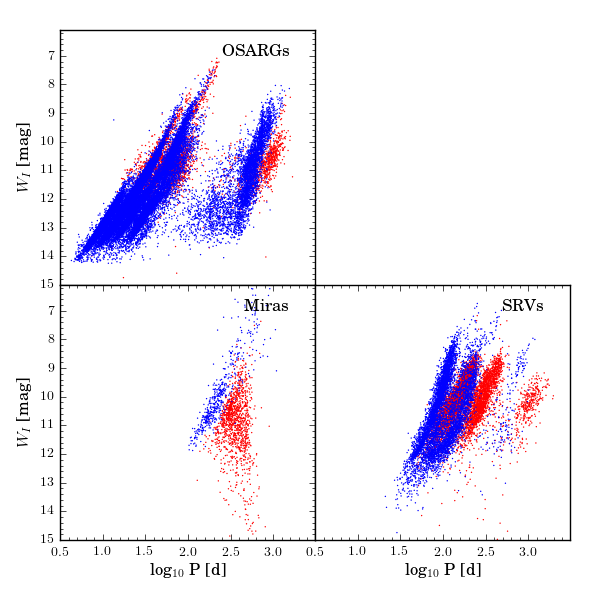
\includegraphics[width=3in]{figs/ogle_2mass_pmag.png}
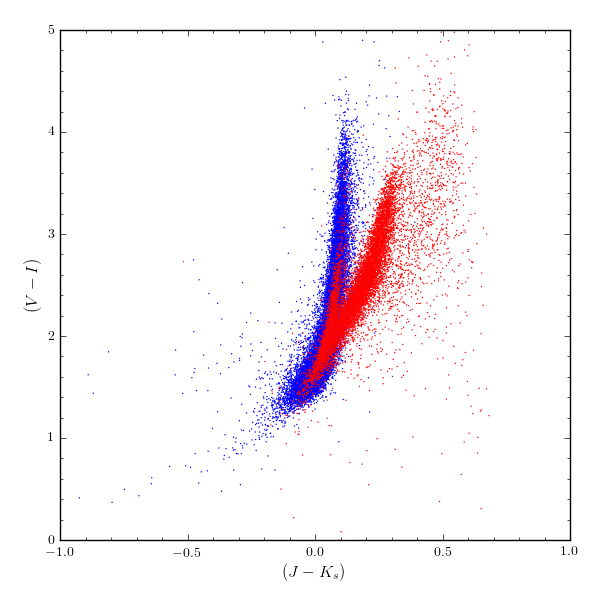
\includegraphics[width=3in]{figs/ogle_2mass_colcol.png}
\caption{Words \label{fig:oglepmag}}
\end{figure}

\subsection{Imaging and spectroscopic catalogs from SDSS}
A few sentences of introduction...
\subsubsection{Galactic sources} 
\subsubsection{Extragalactic populations} 

\subsection{Merged sample}
Each AGB sample as well as the SDSS sources were matched separately to the ALLWISE data products via the {\tt GATOR} tool at the NASA/IPAC Infrared Science Archive\footnote{\url{http://irsa.ipac.caltech.edu/cgi-bin/Gator/nph-scan?mission=irsa&submit=Select&projshort=WISE}}. The accepted matching radius was 3". The matched sample was further reduced by enforcing the WISE 5$\sigma$ faint limits of [$W1/W2/W3/W4$] $<$ [$16.83/15.6/11.32/8.0$], saturation limits of [$W1/W2/W3/W4$] $>$ [2.0/1.5/-3.0/-4.0], signal-to-noise ratios greater than 3 in each WISE band. We constrain the possibility for a mismatched extragalactic IR source by asserting that the extended source flag $\le$ 1, corresponding either to a point source (flag = 0) or a source whose profile-fit photometry is goodness-of-fit is $>$ 3 in any WISE band but is not coincident with any extended sources from the 2MASS survey. We also require only one match to a 2MASS source within 3".

{\color{red}{How was it merged, which further cuts and why...}}


\subsection{Completeness and contamination of the initial \agb\ sample}

In the next section you are using the \agb\ sample from this section to 
estimate completeness and contamination of color-selected samples. Here
you need to summarize what do you believe completeness and contamination
are for your initial sample constructed using SIMBAD and optical surveys.
In particular, it is important to describe expected distance limits. 








\subsection{XXX old stuff from here to the end of this section: Data Sources}
\label{sec:sources}
In this study, we rely heavily on data from the \allwise\, extension of the \wise\, survey, combining data from the initial All-Sky Data Release, the 3-band cryogenic data release, and the NEOWISE post-cryogenic data release \citep{2013wise.rept....1C}. The initial \wise\,All-Sky Data Release observed the sky between January and August 2010, observing the sky 1.2 times with four detectors, operating at 3.4, 4.6, 12, and 22$\mu$m. Hereon we refer to \allwise\, photometric bands at [3.4$\mu$m/4.6$\mu$m/12$\mu$m/22$\mu$m] as [$W1/W2/W3/W4$]. The positions of objects in the \wise\, catalog were calibrated to the \twomass\, point source catalog. The 3-band cryogenic data release contains data from $W1$, 2, and 3, and surveyed $30\%$ of the sky between August and October 2010. During the 3-band cryogenic survey, $W1$ and $W2$ operated with nearly the same sensitivity as during the full survey. Warming of the telescope reduced sensitivity in $W3$ and fully saturated $W4$. The NEOWISE post-cryogenic data release contains $W1$ and $W2$ measurements, with sensitivities close to those obtained during the full cryogenic phase. During this phase, \wise\, surveyed $70\%$ of the sky. Data products from the post-cryogenic release included updated instrumental, astrometric, and photometric calibrations and reduction algorithms, resulting in much lower SNR. The overall number of sources compiled into \allwise\, totals over 747.6 million.

In order to generate a reliable, high-confidence catalog of Galactic candidate \agb\, stars, we must first define color-color criteria from known \agb\, star samples. We select \agb\, stars from three source catalogs: the {\it Optical Gravitational Lens Experiment-III Variable Star Catalog} \citep[\ogle,][]{2008AcA....58...69U,2009AcA....59..239S,2011AcA....61..217S}, the {\it MAssive Compact Halo Objects} project \citep[\macho,][]{1997ApJ...482...89A}, and the \simbad\, Astronomical Database \citep{2000A&AS..143....9W}. 

\ogle\, photometry for Long-Period Variables (LPVs) in the Small and Large Magellanic Clouds (SMC and LMC respsectively) was obtained between July 2001 and May 2009, with stars in the central 4.5-deg$^2$ of the LMC and SMC having an additional 5 observing seasons of photometry from OGLE-II. LPVs were classified into 3 categories: \ogle\, Small Amplitude Red Giants (OSARGs), Semi-Regular Variables (SRVs), and Miras. All AGB stars  O-rich and C-rich \agb\, stars in \ogle\, were photometrically selected using reddening-free Wesenheit magnitudes, described in detail in \cite{2009AcA....59..239S,2011AcA....61..217S}. {\color{red}[Describe the selection bit in a little more detail, along with their sample completeness, selection biases, and contamination fractions]} Data reduction techniques are described in \cite{2008AcA....58...69U}. The resulting samples yield 46,467 \agb\, stars from the LMC (37,203 O-rich; 9,264 C-rich) and 6,509 stars from the SMC (3,727 O-rich; 2,782 C-rich). 

From \macho\, we obtain the sample of SMC, LMC, and Galactic Bulge AGB stars used in \cite{2008AJ....136.1242F} (14,861 stars). {\color{red}Why were these objects selected? Howe were they selected? What is their completeness, selection bias, and contamination fraction?} Following \cite{2008AJ....136.1242F}, the objects are divided into sequences (seq) 1-4. Sequence 1 primarily contains Mira variables pulsating in their fundamental modes, whereas Sequences 2-4 contain semi-regular variables in various pulsation modes.

The sample of AGB stars from \simbad\, was obtained by querying all objects classified as C-stars (18,656), S-stars (1,108), OH/IR stars (825), AGB stars (2,359), and Mira variables (9,608), for a total of 32,556 stars. Objects are classified spectroscopically, though by a variety of methods owing to the heterogeneous data housed within \simbad. Together with \macho\, and \ogle, the total sample of \agb\, stars is 100,393. Because there is a high likelihood that samples between \ogle, \macho, and \simbad overlap, we retain only unique objects after the initial data reduction in section~\ref{sec:reduction}.

We use \sdss\, spectroscopic catalogs to find and quantify regions in NIR-MIR color-color space populated by plausible contaminant sources. These include any Galactic stellar objects and planetary nebulae, as well as a host of extragalactic sources. Data for active galactic nuclei (AGN; 19,184 objects), quasi-stellar objects (QSOs; 122,550 objects), and star forming/burst galaxies (820,272 objects total) were drawn from \sdss\, DR7, specifically from the NYU Value Added Galaxy Catalog\footnote{\url{http://sdss.physics.nyu.edu/vagc/}} \citep[VAGC]{2005AJ....129.2562B}. Luminous Red Galaxies (LRGs) were selected from the SDSS Luminous Red Galaxy Survey \citep[105,631 objects, ][]{2010ApJ...710.1444K}.  Data for stars in the SDSS stellar locus were drawn from the DR 9 SEGUE Stellar Parameters Pipeline (SSPP) \citep[1,843,190 objects, ][]{2012ApJS..203...21A}. {\color{red} Include bit about YSOs and PNe from SIMBAD}

\subsection{Data Reduction}
\label{sec:reduction}
We use NASA/IPAC IRSA's {\tt GATOR} tool\footnote{\url{http://irsa.ipac.caltech.edu/cgi-bin/Gator/nph-scan?mission=irsa&submit=Select&projshort=WISE}} to positionally match \sdss, \ogle, \macho, and \simbad\, to \allwise. We select only matches within 3" between  each sample and \allwise. All samples of \agb\, were required to be brighter than the published 5$\sigma$ faint limits of [16.83/15.6/11.32/8.0], as well as fainter than the saturation limits of [2.0/1.5/-3.0/-4.0] extrapolated from the wings of the PSFs for point sources, for [$W1/W2/W3/W4$] \citep{2013wise.rept....1C}, with no flags for confusion or contamination as a spurious source in any band. We also require only single associations with \twomass\, objects within 3", detections in [$J/K_S/W1/W2/W3/W4$], and SNR $>$ 3 in each \allwise\, band. 

The population for each sample from initial matching as well as after the application of the \allwise\, faint limits, saturation limits, and \twomass\, detection requirements are shown in Table~\ref{tab:pop}. The WISE color-color distributions for the AGB and contaminant samples are shown in Figure~\ref{fig:distros}. \\

\vspace{-10pt}
%\begin{table}[h]
%	\begin{center}
%	\caption{AGB and Contaminant Populations}
%	\scalebox{0.85}{\begin{tabular}{l c c c c c c}
%		\hline
%		Population & SIMBAD C stars & OH/IR stars & Miras & S stars & AGB stars \\
%		\hline
%		2" match & 13,245 & 294 & 8,850 & 1,078 & 1,665 \\
%		Reduced & 3,327 & 165 & 6,218 & 865 & 1,121 \\
%		\hline\hline
%		Population & MACHO seq1 & seq2 & seq3 & seq4\\
%		\hline
%		2" match & 5,193 & 3,441 & 2,548 & 2,931 \\
%		Reduced & 927 & 642 & 263 & 336 \\
%		\hline\hline
%		Population & OGLE C-rich & O-rich\\
%		\hline
%		2" match & 11,417 & 38,369 \\
%		Reduced & 737 & 2515 \\
%		\hline\hline
%		Population & Locus Stars & AGN & LRG & QSO & Galaxies \\
%		\hline
%		2" match & 1,508,158 & 18,481 & 102,178 &  & 799,761 \\
%		Reduced & 168,045 & 9,652 & 7,717 & 18,360 & 125,869 \\
%		\hline
%
%		\label{tab:pop}
%	\end{tabular}}
%	\end{center}
%\end{table}

\begin{table}[h]
	\begin{center}
	
	\scalebox{0.85}{\begin{tabular}{l c c c c c c}
		\hline\hline
		Population & SIMBAD AGB* & C* & Mira & OH/IR & S* \\ 
		\hline
		3" match & 1,689 & 14,209 & 9,027 & 406 & 1,081 \\
		Reduced & 684 & 1,782 & 3,241 & 43 & 511 \\ 
		\hline
		Population & MACHO seq1 & seq2 & seq3 & seq4 \\ 
		\hline
		3" match & 5,279 & 3,519 & 2,619 & 3,070 \\
		Reduced & 277 & 185 & 73 & 61 \\ 
		\hline
		Population & OGLE-III C-rich & O-rich \\ 
		\hline
		3" match & 11,542 & 38,848 \\
		Reduced & 249 & 730 \\ 
		\hline
		Population & DR12 SSPP & DR7 LRG & QSO & AGN & Galaxies \\ 
		\hline
		3" match & 1,578,329 & 104,345 & 103,590 & 18,528 & 841,712 \\ 
		Reduced & 67,508 & 84 & 3,977 & 1,069 & 44,314 \\ 
		\hline\hline

		
	\end{tabular}}    
	\caption{\agb\, and contaminant populations matched to WISE before and after sample reduction in section~\ref{sec:reduction}. MACHO sequences (seq1-seq4) are from \cite{2008AJ....136.1242F} and described briefly in section~\ref{sec:sources}.\label{tab:pop}}
	\end{center}
	
\end{table}

\begin{figure}
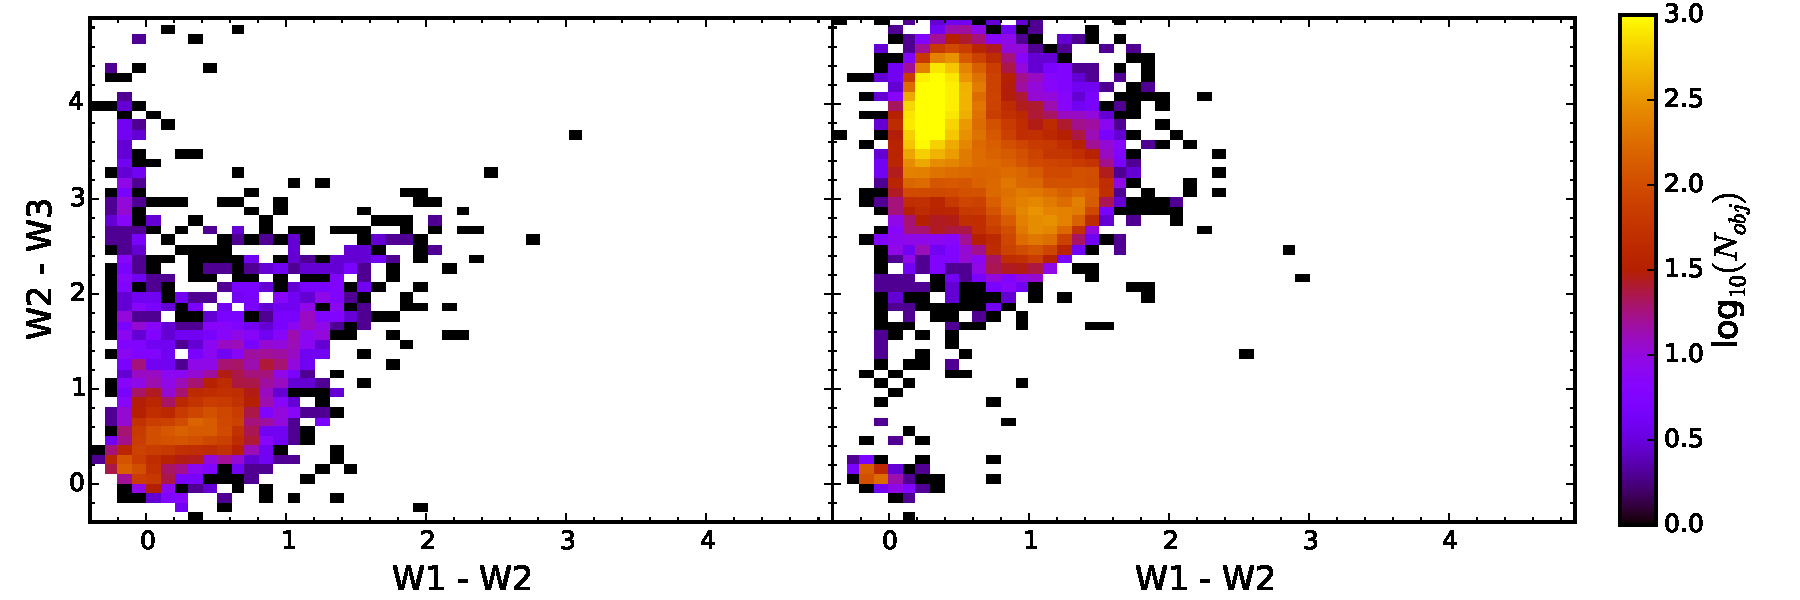
\includegraphics[width=7in]{figs/agbs_contaminants_color_color1.pdf}
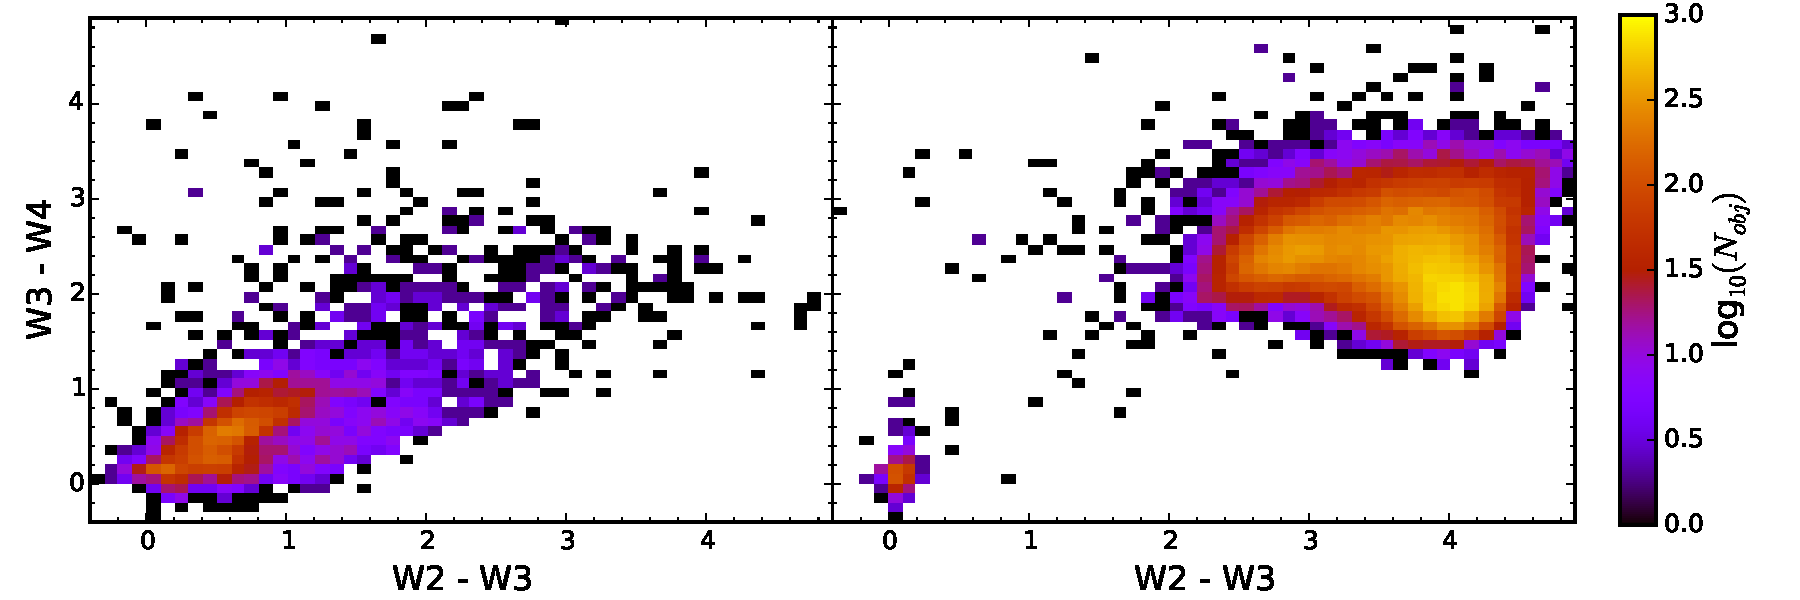
\includegraphics[width=7in]{figs/agbs_contaminants_color_color2.pdf}
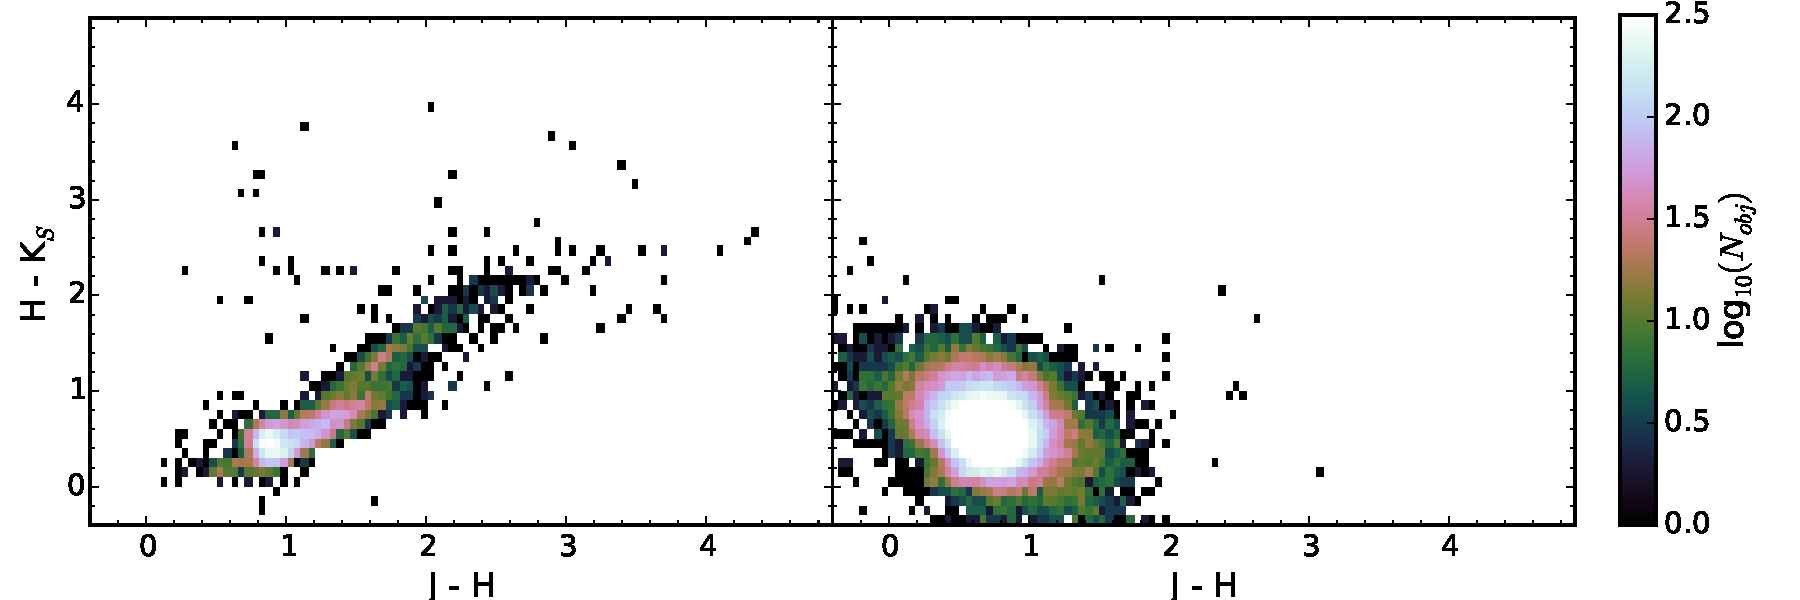
\includegraphics[width=7in]{figs/agbs_contaminants_color_color3.pdf}
\caption{Logarithmic number densities for objects in \wise\, and \twomass\, color-color space, binned in 0.1 dex on each axis. \emph{Left:} The combined AGB sample matched to ALLWISE. \emph{Right:} The combined contaminant sample.\label{fig:distros}}
\end{figure}

